\documentclass[tikz,crop,preview, border=1cm, landscape]{standalone}
  \def\meanOne{0.8}
  \def\meanTwo{0.4}
  \def\binOne{0.7}
  \def\binTwo{0.22}
\usepackage{tikz}
\usepackage{pgfplots}
\begin{document}
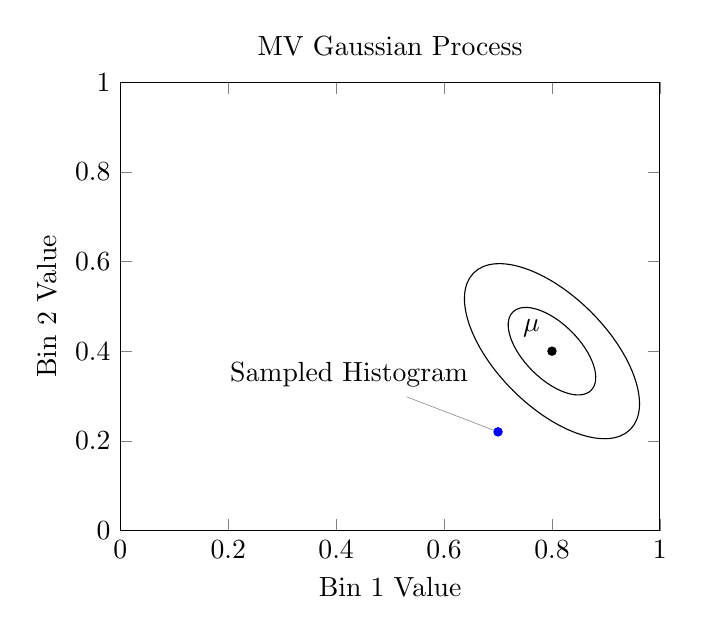
\begin{tikzpicture}
  \def\center{(axis cs: \meanOne,\meanTwo)} 
  \begin{scope}
    \begin{axis}[
      ymin=0, ymax=1,
      xmin=0, xmax=1,
      xlabel={Bin 1 Value},
      ylabel={Bin 2 Value},
      title=MV Gaussian Process]
      \draw[rotate around={45:\center}] \center ellipse (10pt and 20pt); 
      \draw[rotate around={45:\center},] \center ellipse (20pt and 40pt);
      \node[fill=blue, draw=blue,circle, minimum width=3pt, inner sep=0pt,
      pin=120:Sampled Histogram
      ] at (axis cs:\binOne,\binTwo) {};
      \node[fill=black, draw=black,circle, minimum width=3pt, inner sep=0pt, label=120:$\mu$] at \center {};
    \end{axis}
  \end{scope}
\end{tikzpicture}
\end{document}
